\documentclass[13pt,oneside]{book}
\usepackage[utf8]{inputenc}
\usepackage{url}
\usepackage{graphicx}

\usepackage{geometry}
\geometry{a4paper, left=20mm, right=20mm, top=20mm, bottom=20mm}
\usepackage[margin=1.2in]{geometry}
\usepackage[toc,page]{appendix}
\usepackage{graphicx}
\usepackage{natbib}
\usepackage{lipsum}
\usepackage{caption}

\begin{document}

\captionsetup[figure]{margin=1.5cm,font=small,labelfont={bf},name={Figure},labelsep=colon,textfont={it}}
\captionsetup[table]{margin=1.5cm,font=small,labelfont={bf},name={Table},labelsep=colon,textfont={it}}
\setlipsumdefault{1}

\begin{titlepage}
\begin{center}
{\LARGE College Of Engineering Trivandrum}\\[3cm]
\linespread{1.2}\huge {\bfseries Application Software Development Lab}\\[3cm]
\linespread{1}

\includegraphics[width=5cm]{img/emblem.jpeg}\\[3cm]
{\Large GOKUL K\\ S5  CSE \\ Roll No:21\\ TVE18CS021 }\\[1cm]


\textit{ }\\[2cm]
Department of Computer Science\\[0.2cm]
\today
\end{center}

\end{titlepage}

\newpage

\begin{frame}{}
    \centering
    \hspace*{-0.5cm}
    $\vcenter{\hbox{
\includegraphics[width=1.5cm]{img/emblem.jpeg}}}$
    $\vcenter{\resizebox{0.95\textwidth}{!}{
        \begin{tabular}{c}
             CS333 - Application Software Development Lab $\cdot$ 2020 $\cdot$   \\
             \hline 
        \end{tabular}
    }}$
\end{frame}
\section*{Cycle 2}
\section*{Expt 3}
\begin{center}
    \Large{Procedures, Functions and Packages}
\end{center}

\section*{Aim}
\large To study PL/SQL Procedures and functions.

\section*{Experiment}
\begin{itemize}
	\item
Create a function factorial to find the factorial of a number. Use this function in a
 PL/SQL Program to display the factorial of a number read from the user.
 
Syntax:
\begin{verbatim}
CREATE OR REPLACE FUNCTION factorial(N int) RETURNS INT AS $$
DECLARE
        i INT;
        fact INT := 1;
BEGIN
        FOR i IN 1..N LOOP
                fact = fact * i;
        END LOOP;
        RETURN fact;
END;
$$ LANGUAGE plpgsql;

\end{verbatim}
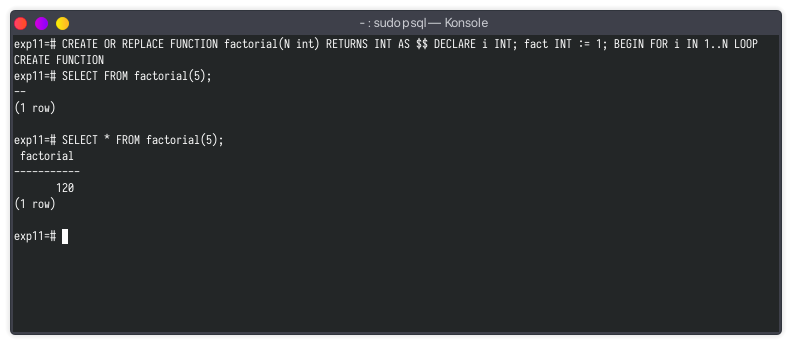
\includegraphics[width=\textwidth]{img/p12/ss1.png}


\item
Create a table student\_details(roll int, marks int, phone int). Create a procedure pr1
 to update all rows in the database. Boost the marks of all students by 5%.
 
Syntax:
\begin{verbatim}
CREATE TABLE student_details (
        roll INT,
        marks INT,
        phone INT
);
INSERT INTO student_details 
VALUES
        (1, 70, 9495969394),
        (2, 60, 8884848584);
CREATE OR REPLACE PROCEDURE pr1()
LANGUAGE plpgsql AS $$
BEGIN
        UPDATE student_details SET marks=marks*1.05;
END;
$$;

\end{verbatim}
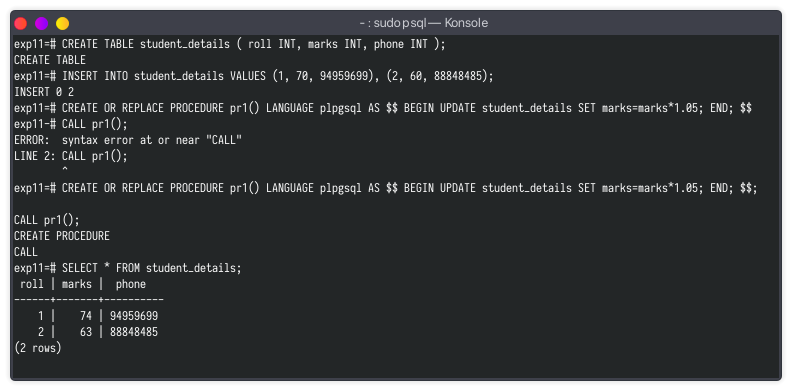
\includegraphics[width=\textwidth]{img/p12/ss2.png}


\item
Create table student (id, name, m1, m2, m3, total, grade). Create a function f1 to
 calculate grade. Create a procedure p1 to update the total and grade.
 
Syntax:
\begin{verbatim}
CREATE TABLE student (
        id INT,
        name VARCHAR(10),
        m1 INT,
        m2 INT,
        m3 INT,
        total INT,
        grade CHAR
);
INSERT INTO student (id, name, m1, m2, m3) VALUES 
        (1, 'NameA', 20, 20, 20),
        (2, 'NameB', 30, 50, 60);
CREATE OR REPLACE FUNCTION f1(total INT) RETURNS CHAR AS $$
BEGIN
        IF total >= 105 THEN RETURN 'A';
        ELSIF total >= 65 THEN RETURN 'B';
        ELSIF total >= 50 THEN RETURN 'C';
        ELSE RETURN 'F';
        END IF;
END;
$$
LANGUAGE plpgsql;
CREATE OR REPLACE PROCEDURE p1()
LANGUAGE plpgsql AS $$
BEGIN
        UPDATE student SET total=m1+m2+m3, grade=(SELECT FROM f1(m1+m2+m3));
END;
$$;

\end{verbatim}
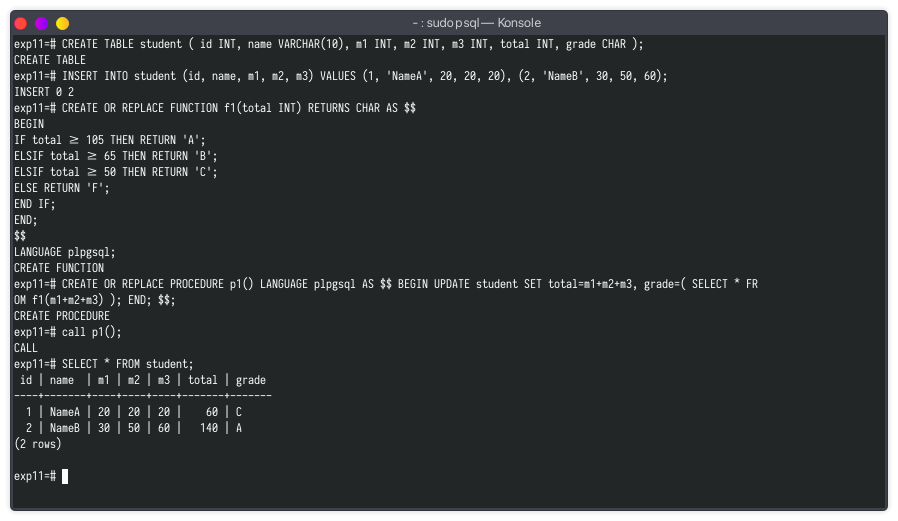
\includegraphics[width=\textwidth]{img/p12/ss3.png}


\item
Create a package (or schema) pk1 consisting of the following functions and
 procedures:
 • Procedure proc1 to find the sum, average and product of two numbers
 • Procedure proc2 to find the square root of a number
 • Function named fn11 to check whether a number is even or not
 • A function named fn22 to find the sum of 3 numbers
 • Use this package in a PL/SQL program. Call the functions f11, f22 and procedures
 pro1, pro2 within the program and display their results

Syntax:
\begin{verbatim}
CREATE SCHEMA pk1;
CREATE OR REPLACE PROCEDURE pk1.proc1(num1 REAL, num2 REAL) 
LANGUAGE plpgsql AS $$
DECLARE
        sum REAL;
        average REAL;
        product REAL;
BEGIN 
        sum = num1 + num2;
        average = sum/2;
        product = num1*num2;
        RAISE INFO 'Sum = %s, Average = %s, Product = %s', sum, average, product;
END;
$$;
CREATE OR REPLACE PROCEDURE pk1.proc2(num REAL)
LANGUAGE plpgsql AS $$
BEGIN
        RAISE INFO 'Root id %s', SQRT(num);
END;
$$;
CREATE OR REPLACE FUNCTION pk1.fn11(num REAL) RETURNS VOID AS $$
DECLARE
        inum INT;
BEGIN
        inum = num;
        IF inum%2 = 1 THEN RAISE INFO '%s is odd', num;
        ELSE RAISE INFO '%s is even', num;
        END IF;
END;
$$
LANGUAGE plpgsql;
CREATE OR REPLACE FUNCTION pk1.fn22(num1 REAL, num2 REAL, num3 REAL) RETURNS VOID AS
$$
BEGIN
        RAISE INFO 'Sum is %s', num1+num2+num3;
END;
$$
LANGUAGE plpgsql;
CREATE OR REPLACE FUNCTION pk1.all(num1 REAL, num2 REAL, num3 REAL) RETURNS VOID AS
$$
BEGIN
        CALL pk1.proc1(num1, num2);
        CALL pk1.proc2(num1);
        PERFORM pk1.fn11(num1);
        PERFORM pk1.fn22(num1, num2, num3);
END;
$$
LANGUAGE plpgsql;
\end{verbatim}
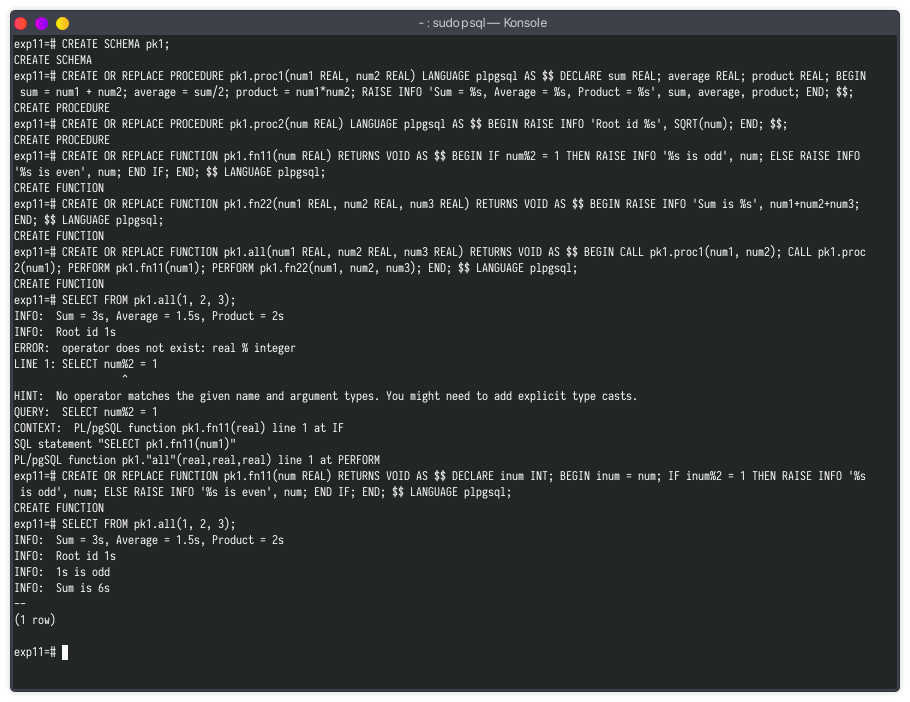
\includegraphics[width=\textwidth]{img/p12/ss4.png}

\end{itemize}
\section*{Result}
	PL/SQL procedures and functions are executed and their output
	is verified in a PostgreSQL environment.
\end{document}